% ================================
% Landon Buell
% Draft 1
% Quantum Physics
% 2 December 2019
% ================================

\documentclass[12pt,letterpaper]{book}
\usepackage{graphicx}
\usepackage{multicol}
\usepackage[left=2.5cm,right=2.5cm,top=2.5cm]{geometry}
\usepackage{array}
%\usepackage{float}
\usepackage{enumitem}
\setitemize{noitemsep,topsep=0pt,parsep=0pt,partopsep=0pt}
\usepackage{amsmath}
\usepackage{physics}
\usepackage{fancyhdr}

% ================================

\pagestyle{fancy}
\fancyhf{}
\rhead{Landon Buell}
\lhead{The Quantum Game}
\cfoot{\thepage}

\begin{document}

% ================================

\title{
\begin{Huge}
The Quantum Game\\
\end{Huge}
\vspace*{5mm}
\Large Applied Elementary Quantum Theory for Non-Physicists}
\author{Landon Buell}
\date{December 2019}
\maketitle


% ================================================================

\begin{center}
--------
\end{center}


\tableofcontents
\pagebreak

% ================================================================

\section*{Introduction}
\paragraph*{}Quantum Physics

% ================================================================

\section*{Preliminary Considerations}

% ================================================================

\section*{Conventions for this Text}

% ================================================================
% ================================================================

\chapter{The Name of the Game}

% ================================================================

\section{The Schrodinger Equation}

\paragraph*{}In classical physics, the description of all motion as we know it, can be in some way attributed to Issac Newton's second law of motion, which tell us that the force acting on an object is equal to the objects mass, multiplied by the acceleration of the object. More conveniently written: $F = ma$. Or rather:
\begin{equation}
\label{Newtons 2nd Law}
F = m\frac{d^2x}{dt^2}
\end{equation} 
in more mathematically expression. Where $x$, or rather $x(t)$ is a time dependent function that describes the motion of the object in a single spatial component.
\paragraph*{}The forces acting on any arbitrary object in question can be equated to $m\frac{d^2x}{dt^2}$ and the resulting differential equation can be solved to find the function $x(t)$, that tracks the position of the object with time. Admittedly, this proves to be quite difficult in some cases and literally impossible in other cases. Luckily for us, in the 21st century, we have the ability to use computers and have the benefit of numerical problem solving which will come in heady later on.
\paragraph*{}In quantum physics, we don't have such a nice, clean equation as Sir Newton has laid out for us, but a much, much messier one that behaves in a similar way. It was created around 1925 by the Austrian Physicist, \textit{Erwin Schrodinger}. It looks something like:
\begin{equation}
\label{1D Schrodinger}
-\frac{\hbar^2}{2m}\frac{\partial^2\Psi}{\partial x^2} +
V\Psi = i\hbar\frac{\partial \Psi}{\partial t}
\end{equation}
\paragraph*{}Everything about modern quantum physics in some way, either comes from, or comes back to this equation. Just like in classical physics, all motion is attributed to Newton's second law of motion, equation (\ref{Newtons 2nd Law}), in quantum physics, all properties of the quantum system are attributed to Schrodinger's equation, (\ref{1D Schrodinger}).

% ================================

\paragraph*{}Consider a point particle, of some mass, $m$, constrained to move along a one-dimensional, line, which we will conveniently choose to be the $x$-axis. If we know the mass, and the particles position as a function of time, $x(t)$ we can deduce several other properties of the system. By taking the derivative of $x(t)$ with respect to time, we can detemine the particles velocity all time, $v(t)$. Here, we can compute the kinetic energy $\frac{1}{2}mv^2$ and momentum $mv$ at all points in time. Taking another time derivative gives us the acceleration of the particle at all time, $a(t)$. From there, we can find the force $ma$ and the even the potential energy function at all times. 
\paragraph*{}Just by simply knowing the mass and position function for an object grants a great deal of information to you. We can find position, velocity, acceleration, force, energy, momentum and so many of these important dynamical variables by doing some simple bits of calculus or algebra. In all cases, we can evaluate these little formulas at any point in space or time to find \textit{exactly} the value we want. Classical physics operates under this assumption, that we can accurately describe the world around us and it behaves according to these mathematical descriptions.
\paragraph*{}Quantum physics holds a different sent of requirements from us however. Things tend to not be so well defined. Rather than being able to calculate or measure the \textit{exact} value of the quantity that we want, we are forced to only be able to determine a \textit{probabilistic} value of what we want. In other words, things are not entering values and parameters to find for \textit{certain} what we want, but instead quantum physics becomes a game of \textit{probability}.
\paragraph*{}This business of probability, called the \textbf{statistical interpretation} comes with it the idea of \textit{uncertainty} and \textit{ambiguity}. Our entire understanding of the macro universe relies on the idea that things are exactly measurable and perfectly determinant, but the universe on a quantum level cannot be described with anything more than statistics. And, as we'll see very shortly, it is this statistical information which shapes our understanding of the subject entirely - the fact that we can only talk about the \textit{possible} results that happen with a certain \textit{probability}. This lack of certainty is what is so strikingly dreadful about this field and has been source for countless restless nights over the decades. This poses the currently unanswerable question that arises: is this nature is a product of the universe or a product of our mathematical treatment? 
\paragraph*{}Probability is \textit{the name of the game} of quantum physics. The mechanics of a quantum system are not defined by a mass $m$ and a position function, $x(t)$, but rather are defined by a probability amplitude function, \textit{the wave function}, $\Psi(x,t)$ which is represented by the Greek letter Psi, and appears three times in the Schrodinger equation above.
\paragraph*{}This function, $\Psi(x,t)$, or often just $\Psi$, contains with it all possible information about a quantum mechanical system. With the wave function $\Psi$ known, we can determine the relative probabilities of position, momenta and other system parameters. For example, the expression:
\begin{equation}
\label{prob_ab}
\int_a^b \big | \Psi(x,t) \big|^2 dx
\end{equation}
gives the probability of finding some particle on the $x$-axis between the values of $a$ and $b$ at some fixed time $t$. This business of probability is called \textit{The Statistical Interpretation} of Quantum Mechanics and is arguable the largest underlying points in quantum theory - that our entire model is based on statistically described behavior.
\paragraph*{}But how exactly do we \textit{get} $\Psi(x,t)$? In Classical physics, we get $x(t)$ often by solving a second-order ordinary differential equation from Newton's laws. In Quantum physics, we get $\Psi(x,t)$ by solving the second-order, partial differential equation - Schrodinger's equation. As with classical physics, this tends to be a bit messy and often not really reasonable to do by hand- at least not without understanding some other concepts first. So, before we go off trying to \textit{solve} equation (\ref{1D Schrodinger}) for the wave function, $\Psi$ we must understand a little bit more about it first - what does it mean?


% ================================================================

\section{The Wave Function}

\paragraph*{}Before we construct a means to finding this mysterious function, $\Psi(x,t)$ and treating it mathematically, we need to produce a more concrete understanding of what this function is trying to \textit{tell} us. Outside of pure mathematics, we need a motivation to play this part of the game and It's such an important characteristic of quantum physics that we cannot afford to not set aside some time to understand how it works.
\paragraph*{}In one sentence: The wave function is a probability \textit{amplitude} for finding a particle in some space, at some time. A common misconception is that the wave function itself is the probability \textit{density} is in correct. It is the quantity of: $\Psi^*(x,t) \Psi(x,t)$ that gives the actually probability density of finding a particle at a space and a time. With this, we can equate this to a probability function:
\begin{equation}
\label{prob density func}
\Psi^*(x,t) \Psi(x,t) = \big | \Psi(x,t) \big|^2 = P(x,t)
\end{equation}
\paragraph*{}Then, as shown in equation (\ref{prob_ab}), integrating this function over some spatial region, from $a$ to $b$, gives the probability of finding a quantum particle, with the wave function, $\Psi(x,t)$, between the region $a$ and $b$. Naturally, integrating this function over all of space, (i.e., $-\infty$ to $+\infty$) would identically produce the result $1$. Physically, this is a result of the fact that the particle must exists \textit{somewhere} in all of space, so the chances of finidng it with the region of infinity must be $1$.
\paragraph*{}This is raises the problem  that most functions, when integrated over all of space, do \textit{not} produce a value of $1$. So, whenever we fins the wave function for a particle, we must first \textit{normalize} it's area to $1$. This means, that we must find a normalization constant $A$ that satisfies the equation:
\begin{equation}
\label{normalize wave function}
1 = A\int_{-\infty}^{+\infty} \big | \Psi(x,t) \big|^2 dx
\end{equation}
\paragraph*{}Once we've found this normalization constant, $A$, we can evaluate the integral at various bounds to find the probability (out of 1) of find the particle in that regions. For Example if you found the result:
\begin{equation}
A\int_{c}^{d} \big | \Psi(x,t) \big|^2 dx = 0.35
\end{equation}
and assuming the interval $[c,d]$ is not all of space, then there is a 35\% chance of find the particle between the region $c$ and $d$ at some time $t$.This statistical interpretation comes with some other rules that may be worth writing out. Many of which some from simple calculus rules of integration.

\begin{enumerate}
\item[•]\textbf{Probability:}\\
A normalized wave function has the property
\begin{equation}
A\int_{a}^{b} \big | \Psi(x,t) \big|^2 dx \leq 1
\end{equation}
There is never more than a 100\% chance of finding a particle over any interval, and that a particle must exist somewhere in a region. If the system demands that the particle can only be in the region $a$ and $b$, then the integral over that region must be equal to $1$. Additionally, once a particle is normalized at a time $t$, it is also normalized for all time as well.
\item[•]\textbf{Addition of Probability:}\\
If a region of space divided into $N$ segments, the sum of the probabilities of finding the particles in each regions must be equal to finding the total probability of the while region.
\begin{equation}
\int_{a_0}^{a_N} \big | \Psi(x,t) \big|^2 dx =
\int_{a_0}^{a_1} \big | \Psi(x,t) \big|^2 dx + ... +
\int_{a_{N-1}}^{a_N} \big | \Psi(x,t) \big|^2 dx
\end{equation}
\item[•]\textbf{Zero Probability}\\
The particle odds of a particle being \textit{exactly} at are point $b$ are identically \textit{zero}. From calculus, when integrating a function over a region $b$ to $b$ the result is always zero independent of a the function, time or normalization. 
\begin{equation}
\int_{b}^{b} \big | \Psi(x,t) \big|^2 dx = 0
\end{equation}
\end{enumerate}
\paragraph*{}Aside from purely mathematical objects, $\Psi(x,t)$ must also have some physical properties - otherwise Quantum Physics would be purely Quantum Mathematics. This forces us to consider some other parameters that are not explicitly expressed from the mathematics.

\begin{enumerate}
\item[•]\textbf{Normalizeable}\\
Wave function must be normalizeable. When we actually solve the Schrodinger equation, it must be a function that can be normalized. Otherwise, our statistical interpretation breaks down, and we find ourselves in trouble. For example, the function $\Psi(x,t) = 0$ is a valid solution to the partial differential equation, but it cannot the normalized over all of space. 
\item[•]\textbf{Continuity}\\
Wave functions must be continuous and continuously differentiable when subject to potentials that are also continuous are continuously differentiated. This means that if a potential function, $V(x)$ is perfectly continuous, so must the resulting wave function. Only in cases where potentials are discontinuous (i.e. peice-wise defined) can the function and it's first derivative be discontinuous.
\end{enumerate}

\paragraph*{}Believe it or now, we now have a very solid basis for what the wave function actually is and how it works. 

% ================================================================

\section{Breaking Down the Schrodinger Equation}
\paragraph*{}If the name of the game in quantum physics is understanding probability densities and statistical behavior of systems, then the game is played by finding that probability function. This means to solve the Schrodinger equation for $\Psi(x,t)$, which gives the \textit{probability amplitude} and multiplying it by it's own \textit{complex conjugate}. This takes the form of $\Psi^*\Psi$ or the integrand of equation (\ref{prob_ab}).
\paragraph*{}At first glance, the equation:
\begin{equation}
\label{1D Schrodinger expanded}
-\frac{\hbar^2}{2m}\frac{\partial^2}{\partial x^2}\Big[ \Psi(x,t) \Big] +
V(x)\Psi(x,t) = i\hbar\frac{\partial}{\partial t}\Big[ \Psi(x,t) \Big]
\end{equation}
whichs is just equation (\ref{1D Schrodinger}) expanded out a little bit, has a lot of information to unpack, even for a seasoned user of mathematics. For this section, we're going to try to determine what this equation is actually trying to tell us, and what each peice of it means. First off, lets take it apart, one tedious variable at a time. 
\paragraph*{}The value $\hbar$ is defined as $\frac{h}{2\pi}$ where $h$ is \textit{Planck's constant}. $\hbar$ itself happens to be a more useful quantity in quantum mechanics, it has a value of $1.054573\times 10^{-34}$ Joule-seconds. The parameter $m$ is the mass of the particle in questions. When put together, the term $-\frac{\hbar^2}{2m}$ is simply a scalar value -i.e. it's just a number, a constant coefficient.
\paragraph*{}The term $V(x)$ represents the \textit{potential function} of the quantum mechanical system. In almost all case, it will \textit{just} be a function of space, \textit{not} time- although this is not always the case. This describes the potential energy distribution as a function of space along our one-dimensional system. When it comes to solving equation (\ref{1D Schrodinger expanded}), this is really the limiting factor in what determines the shape of the solution, as we'll see in chapter 2.
\paragraph*{}The partial derivatives of $\Psi(x,t)$ are a little bit tougher to reason out, but they are very akin to the mechanics of the heat equation where a second spatial derivative is proportional to a first time derivative. In a little while we'll see how this relationship allows for some nice simplifications to be made.
\paragraph*{}Now that We've broken down each part of the equation, we can begin to formulate an analytical solution. This in practice need only be done once because, where we will end up is a convenient starting place for the rest of all calculations to be done. As stated before, the goal of solving this partial differential equation (or PDE for short) is to find $\Psi(x,t)$, a function of both space, $x$ and time, $t$. To do this, we will assume that $\Psi(x,t)$ is a composition, or the product of two 'smaller' functions, one of just space, and another of just time. This means that $\Psi$ can be broken down into a spatial function, which we'll call $\psi(x)$ and a temporal function, which we'll call $\phi(t)$. This then allows for the very import relation that will come back to haunt us over and over again:
\begin{equation}
\label{separable}
\Psi(x,t) = \psi(x)\phi(t)
\end{equation}
\paragraph*{}The exact reasoning for this is quite unclear at first, and that's okay for now- it's use will become apparent later on. This new form for our equation allows us to write equation (\ref{1D Schrodinger expanded}) as:
\begin{equation}
\label{separated TDSE 0}
-\frac{\hbar^2}{2m}\frac{\partial^2}{\partial x^2}\Big[ \psi(x)\phi(t) \Big] +
V(x)\Big[ \psi(x)\phi(t) \Big] = i\hbar\frac{\partial}{\partial t}\Big[ \psi(x)\phi(t) \Big]
\end{equation}
\paragraph*{}We can use the linear properties of the derivative operator to further help us out. Functions of time are not affected under a spatial derivative, and functions of space are not affected under a temporal derivative. This lets us conveniently remove those untouched functions as such, and use some short hand. $\psi(x)$ becomes $\psi$ and $\phi(t)$ becomes $\phi$.
\begin{equation}
\label{separated TDSE 1}
-\frac{\hbar^2}{2m}\phi\frac{\partial^2\psi}{\partial x^2} +
V\big[ \psi\phi \big] = 
i\hbar\psi\frac{\partial \phi}{\partial t}
\end{equation}
\paragraph*{}Lastly, we can divide both sides of the equation by $\psi(x)\phi(t)$. Now, equation (\ref{separated TDSE 1}) becomes:
\begin{equation}
\label{separated TDSE 2}
-\frac{\hbar^2}{2m}\frac{1}{\psi}\frac{\partial^2\psi}{\partial x^2} + V = 
i\hbar \frac{1}{\phi}\frac{\partial \phi}{\partial t}
\end{equation}
\paragraph*{}Now, we can all functions of \textit{space} on the left side, and all functions of \textit{time} on the right side. In order for both sides of this equation to be equal for \textit{all of 1D space} and \textit{all of time}, they must be identically constant. This fact is tough to grasp and it's true comprehension may have to be saved for another text, but in reality it is this mathematical rule that motivates us to choose the separable solution form in equation (\ref{separable}).
\paragraph*{}If we examine just the right side, the time function's side, we can set it to an 'arbitrary' constant $E$ - for reasons we'll discover later. Now we can write:
\begin{equation}
\label{energy ODE}
E = i\hbar \frac{1}{\phi}\frac{d\phi}{dt}
\end{equation}
\paragraph*{}This time dependent ODE, (\ref{energy ODE}) can be conveniently solved with it's own separation technique to see that the function, $\phi(t)$ is really:
\begin{equation}
\label{phi}
\phi(t) =  e^{-i\frac{E}{\hbar}t}
\end{equation}
\paragraph*{}Note that the partial derivatives are now full derivatives, which is again a product of this separation technique. We can put this new constant, $E$, back into the right side of equation (\ref{separated TDSE 2}) and then multiply again by $\psi(x)$. The result is something new, but familiar:
\begin{equation}
\label{TISE}
-\frac{\hbar^2}{2m}\frac{d^2\psi}{dx^2} + V(x)\psi(x) = E\psi(x)
\end{equation}
\paragraph*{}This is called the \textbf{Time Independent Schrodinger Equation} (TISE). This equation, (\ref{TISE}) is the convenient starting place for rest of the procedures in this text - and works consistently provided that the potential function, $V$ does \textit{not} change with time. By using this separation of variables technique, we have turned the full Schrodinger Equation, (\ref{1D Schrodinger expanded}), a\textit{partial} differential equation, into two separate, \textit{ordinary} differential equations, 
(\ref{energy ODE}) and  (\ref{TISE}). 
\paragraph*{}It is important to know as well that using separation of variables provides an infinite set of solutions to the PDE. There are infinitely functions $\psi(x)$ that satisfy the equation given the way we have chosen to solve it. Furthermore, the separation technique, where $\Psi(x,t) = \psi(x)\phi(t)$ is only a part of the picture - for example one could choose to look at solutions of the form $\Psi(x,t) = \psi(x) + \phi(t)$ which would in turn provide another set of infinite solutions. 
\paragraph*{}The separation technique does however allow for some convenient properties:
\begin{enumerate}
\item[•]\textbf{General Time Dependence}\\
Despite not having this function exactly, at the moment, we can still do a lot with the information that we currently have. We have established that the time portion is \textit{not} dependent on the potential, so that whenever we do fine $\psi(x)$, we can simply multiply the same function, (\ref{phi}) time any spatial solution. Thus any full solution as a form:
\begin{equation}
\Psi(x,t) = \psi(x)e^{-i\frac{E}{\hbar}t}
\end{equation}
\item[•]\textbf{Linear Combination}\\
The Schrodinger equation is a \textit{linear} partial differential equation. This means that a linear combination of known solutions is \textit{also} a valid solution as well. So, if we have a collection of solutions scaled by some constant,
$c_1\psi_1(x)$ , $c_2\psi_2(x)$ , ... , $c_N\psi_N(x)$, etc., adding them all together is yet \textit{another} possible wave function. Thus now, any $\Psi(x,t)$ actually can be expressed as:
\begin{equation}
\label{linear combo}
\Psi(x,t) = \sum_n^{\infty} c_n \psi_n(x) \phi_n(t)
\end{equation}
Notice how $\phi(t)$ also changes with $n$, we will explore this in a little while. 
\item[•]\textbf{Probability Density}\\
The complex exponential in the time function eliminates itself when multiplied by it's own complex conjugate. When we compute $\big | \Psi(x,t) \big|^2$, the quantity $e^{-i\frac{E}{\hbar}t}e^{+i\frac{E}{\hbar}t}$ becomes just $e^0 = 1$. Thus the time component does not affect our normalization constant from before. 
\end{enumerate}

\paragraph*{}The bulk of chapter 2 will be dedicated to solving equation (\ref{TISE}) for very specific potential functions, $V(x)$ and why they are so important. 
\paragraph*{}In short, we now have a more digestible way of handling quantum physics. What we've done here, is a means to an ends - or rather a means to a beginning of \textit{playing} the game and quantum mechanics. While our treatment of the subject so far is \textit{purely} mathematical, it's important to understand that it's very important to playing out the ground work for the rest of the subject. 

% ================================================================

\section{The Language of the Game}
\paragraph*{}As you can see from the previous sections of this chapter, quantum physics is very much a mathematically heavy topic. In classical physics, we can make qualitative observations of the universe and then build mathematical models around those observations. Early on, we established that Newton's 2nd Law, equation (\ref{Newtons 2nd Law}) becomes a dominant figure in the field and such second order, ordinary differential equations become the language of classical physics.
\paragraph*{}In quantum physics, the Schrodinger Equation, (\ref{1D Schrodinger}) is the dominant figure,a and it would make such that second order partial differential equations become the language of quantum physics. As strange as it may sound, the dominant set of tools used for the mathematics of quantum mechanics is mostly based in \textit{linear algebra}.
\paragraph*{}Linear algebra is a type of mathematics that deals largely with vectors, matrices and the idea of spaces and dimensions. However, English physicist Paul Dirac used principles from linear algebra to build in part, his own system of notations designed especially for handling the mathematics of quantum physics. In reality, this system of notation is not essential for quantum physics, but instead allows us to simplify a great deal of concepts, and convey information in a new way.
\paragraph*{}I shall assume that you are familiar with linear algebra, if not on a fully function level, at least in concept. As dense as a next few sections of read may be, it's important to remember that functionally, all of the math in quantum is just as you've been taught in the past, only expressed differently. In order to introduce each piece and rule of notation, I'll describes it's relation and origin from linear algebra as well.

% ================================

\subsection*{Vectors, and Bras and Kets}
\paragraph*{}A vector is a mathematical object that allows very simply to communicate the dimension, components, magnitude and orientation of a measurement all very conveniently. Typically, a vector is notated as a variable with a little arrow on top such as $\vec{\psi}$. The vector is then made up of $N$ discrete components. They can be written out in columns or rows, for example:
\begin{equation}
\label{vector}
\vec{\psi} = \big[ a_0 , a_1 , \hdots , a_N ] =
\begin{bmatrix}
a_0 \\ a_1  \\ \vdots \\ a_N
\end{bmatrix}
\end{equation}
\paragraph*{}The number of components, $N$ indicates the dimension of the vector, i.e., it is $N$-dimensional. The entry in each index represents the length or \textit{measure} of the vector in that particular component. Note that each entry, $a_n$ can be a real, imaginary or complex value. In quantum mathematics, we replace the linear algebra object of a vector with the \textit{new} mathematical object called a \textit{ket}.
\begin{center}
A ket is notated as $\ket{\psi}$ 
\end{center} 
and has many of the same properties as a vector.
\paragraph*{}Just like a vector, a ket exists in a space, has components and can interact with other mathematical objects. It shares almost all of the same properties as vectors. A ket can be modified by a (real, imaginary or complex) scalar value. A ket can also be multiplied by a matrix (which we'll call an \textit{operator} later) to produce another ket. They can compared to other kets with dot product and cross produces and can be arranged into linear combinations as well.
\paragraph*{}In addition to the ket, there is a related mathematical object called a \textit{bra} which has all of the same properties as a ket.
\begin{center}
A bra is notated as $\bra{\psi}$
\end{center}
The relationship between bras and kets is simply that they are eachother's \textit{complex conjugates}. More mathematically, a bra is this \textit{dual space} counterpart to the ket vector space, and vice-versa. This means that:
\begin{equation}
\bra{\psi} = \ket{\psi}^* 
\text{\hspace*{8mm} and \hspace*{8mm}} 
\ket{\psi} = \bra{\psi}^*
\end{equation}
Every ket has a corresponding bra, and every bra has a corresponding ket.
\begin{equation}
\ket{\psi} \longleftrightarrow \bra{\psi}
\end{equation}

\paragraph*{}Suppose for example is the ket $\ket{\alpha}$ is defined by $N$ real, imaginary or complex discrete components:
\begin{equation}
\label{discrete ket}
\ket{\alpha} \equiv
\begin{bmatrix}
(a + ib)_0 \\ (a + ib)_1 \\ \vdots \\ (a + ib)_N
\end{bmatrix}
\end{equation}
Then it's dual space, or bra equivalent, $\bra{\alpha}$ is then defined as it's  complex conjugate:
\begin{equation}
\label{discrete bra}
\bra{\alpha} = 
\ket{\alpha}^* \equiv
\begin{bmatrix}
(a - ib)_0 \\ (a - ib)_1 \\ \vdots \\ (a - ib)_N
\end{bmatrix}
\end{equation}

\paragraph*{}There are some important distinctions between vectors, kets and bras that need to be outlined as they are not the same thing. Vectors typically have a finite number of components in them, and thus are limited to finite dimensional vector spaces. A ket or bra on the other hand, can potentially have an infinite amount of components in it. Where a vector is a set of discrete indexes, a ket or bra can thought of as a set on continuous set of values. Furthermore, a ket or bra can be used to express a function, or rather the output of a function. For example, a ket with infinite entries can be used to convey the output of a single, smooth, and continuous function.
\paragraph*{}For example, the ket, $\ket{\beta}$ could be used to represent the continuous output for the complex defined function:
\begin{equation}
\label{smooth ket}
\ket{\beta} \equiv (a + ib) e^{-i\omega t}
\end{equation}
Then it's dual space, or bra equivalent, $\bra{\beta}$ is again defined as it's  complex conjugate: 
\begin{equation}
\label{smooth bra}
\bra{\beta} \equiv (a - ib) e^{+i\omega t}
\end{equation}

\paragraph*{}Computationally, vectors and kets are handled in the exact same way because a computer cannot convey an infinite number of points to produce a line or function. Rather, they are limited to holding a discrete number of values. Because of this, vectors, kets and bras are all handled mostly as list or array - like mathematical objects. After all, they hold many of the same properties are can \textit{often} be used interchangeably. If the notation $\bra{\psi}$ or $\ket{\psi}$ ever confuses you, just remember that are \textit{functionally vectors} with certain additional properties.

% ================================

\subsection*{Inner Products and Bra-Kets}

\paragraph*{}It may come as no surprise that Paul Dirac just the names "bra" and "ket" together. Very cleverly, and perhaps humorously, when they combine, they create a mathematical operation of the \textit{dot product} (often also called scalar product or inner product). Image two discrete vectors, 
$\vec{eta}$ and $\vec{\xi}$, both of length $N$. The dot product between them is defined as:
\begin{equation}
\label{dot product}
(\vec{\eta} \cdot \vec{\xi}) \equiv \sum_{i=0}^N (\vec{\eta}_i)(\vec{\xi}_i)
\end{equation}
In words, each index of one vector is multiplied by that same index in the other vector, and then each product is summed to output a single scalar number, real or complex.
\paragraph*{}The Dirac equivalent is the \textit{inner product} and is notatied by the combination of a bra and ket, conveniently called a \textit{bra-ket}.
\begin{center}
A bra-ket is notated as $\braket{\psi}{\psi}$
\end{center}
Just like before, if the bra and ket are both discretely defined, $\bra{\eta}$ and $\ket{\xi}$, then then inner product of them is similar to equation (\ref{dot product}), except with the added complex conjugate:
\begin{equation}
\label{comp-conj dot product}
\braket{\eta}{\xi} \equiv \sum_{i=0}^N (\eta^*_i) (\xi_i)
\end{equation}
\paragraph*{}Conversely, if a ket and bra are both continuously defined functions of $x$, $\bra{f(x)}$ and $\ket{g(x)}$ as in (\ref{smooth ket}) and (\ref{smooth bra}), then the inner product takes as lightly modified form. The discrete sums from equation (\ref{comp-conj dot product}) now becomes a continuous, infinite sum, \textit{an integral}! So, the inner product of $f(x)$ and $g(x)$ (on the basis of $x$) now becomes:
\begin{equation}
\label{bra-ket}
\braket{f(x)}{g(x)} = \int f^*(x) g(x) dx
\end{equation}
\paragraph*{}Furthermore, harking back to the wave function directly, we can use this new concept and notation to help. With the wave function, $\Psi(x,t)$, found, then we can write the probability density for the system, given in equation (\ref{prob density func}), as an inner product.
\begin{equation}
\label{inner prod integral}
\braket{\Psi}{\Psi} = \int \Psi^*(x,t) \Psi(x,t) dx
\end{equation}

\paragraph*{}In the conventional notation for quantum physics, this is usually the standard way of expressing the probability density for a particle, given a wave function. This also usually comes with the implication that the function is already normalized, i.e. the constant $A$ has been absorbed into the inner product such that it alone is equal to 1:
\begin{equation}
\braket{\Psi}{\Psi} = 1
\end{equation}
\paragraph*{}It is also important to note that the properties of bras and kets are preserved in the inner product operation as well. For example, the complex conjugates of an inner product has the property:
\begin{equation}
\braket{\psi}{\phi}^* = \braket{\phi}{\psi} 
\end{equation}
Where the complex conjugate operation is applied to $\bra{\psi}$ and to $\ket{\phi}$ to becomes $\ket{\psi}$ and $\bra{\phi}$ respectively.
\paragraph*{}And all of these relations for bras and kets hold true with the analog to vectors. For example, a set of three orthogonal basis vectors in 3D Cartesian space may define a coordinate system, just as three orthogonal kets or bras may be used to define the space or coordinate system. A linear combination of kets is also a valid concept, such as equation (\ref{linear combo}) would take the form:
\begin{equation}
\label{linear combo kets}
\Psi(x,t) = \sum_n^{\infty} c_n \ket{\psi_n(x)}\phi_n(t)
\end{equation}

% ================================

\subsection*{Matrices and Operators}
\paragraph*{}Another important tool from linear algebra is the \textit{matrix} object. In some ways, a matrix is a concatenation of various column or row vectors that together produce a square or rectangular grid of entries. This matrix can object thought of as a \textit{linear operator}- a mathematical object that takes some object - a vector (or a ket) and turns it into another object - another vector (or ket).
\paragraph*{}In quantum physics, this matrix concept is extremely important - but instead of being a matrix with finitely many components and entries, it is called an \textit{operator} that has potentially infinity many entries. Because of this, a matrix in linear algebra becomes an operator in quantum physics.
\begin{center}
An operator is notated as $\hat{Q}$
\end{center}
\paragraph*{}Just like before, this operator now posses some neat intrinsic qualities. An $N \times M$ matrix $A$ could take a $M \times 1$ vector, $\vec{v}$ anf transform it into a $N \times 1$ vector, $\vec{w}$ - given by the matrix vector equation:
\begin{equation}
\label{mat-vec}
\vec{w} =  A\vec{v}
\end{equation}
Would then become:
\begin{equation}
\label{op-ket}
\ket{w} = \hat{A}\ket{v}
\end{equation}
Where all elements could be either finitely dimensional on infinitely dimensional.
\paragraph*{}It is important to note that in Dirac notation of quantum mechanics, operators, unless notated otherwise act on the object to the \textit{right} of them.

% ================================

\subsection*{Probability}

% ================================================================

\section{The Characters in the Game}

% ================================


\subsection*{Spaces and Basis}
\paragraph*{}One of the strangest concepts from quantum physics and linear algebra is the idea of \textit{spaces}. 


% ================================

\subsection*{Position Space}
\paragraph*{}Position space, also referred to the \textit{position basis} functions as a system of measurement.


% ================================

\subsection*{Momentum Space}

% ================================

\subsection*{Hilbert Space}
 
% ================================================================

\section{The Eigenvalue Problem}

% ================================================================

\section{Takeaways from this Chapter}

% ================================================================
% ================================================================

\chapter{Playing the Game: \\ Quantum Physics in 1 Dimension}

% ================================

\paragraph*{}This chapter of this text will be devoted to applying what we've learned about the basic and the mathematical behavior of quantum physics to specific potential cases in one spatial dimension. Over the course of this chapter, the specific potential cases examined are very similar to cases explored in other quantum texts. This similarity is due to the interesting cases, and important lessons that arise from each possible potential function. It is important to take all of this with a grain of salt, however as these are obviously over-idealized circumstances, that need to be heavily expanded upon before becoming of any real-world use or application.
\paragraph*{}For this chapter, the 1-Dimensional Time Independent Schrodinger Equation (1D TISE) will be the starting place for each particular case, as we will assume to that all of these potentials exist on a single, infinitely long line, and remain constant with time. The 1D TISE is again:
\begin{equation}
\label{1D TISE}
-\frac{\hbar^2}{2m}\frac{d^2 \psi}{dx^2} + V(x)\psi = E\psi
\end{equation}
Which can aslo be written in it's operator eigen value form:
\begin{equation}
\label{1D TISE Eigen}
\hat{H}\ket{\psi} = E\ket{\psi}
\end{equation}
\paragraph*{}In Each potential case, as part of the nature of this text, I will discuss the methods used in numerically solving the Schrodinger equation. As modern the complexity of modern science and engineering increases, it becomes more obvious that the ability to solve such a complicated partial differential equation is an effort in faultily.Because of this, I will present the analytical solution to the equation, as it would be solve by hand, and than compare that result to something produced numerically. This way, you have a mathematical foundation to sit upon and a more reasonable way to go about solving any arbitrary quantum system. This of course is not to discredit the hard work of pre-computation physicists and mathematicians, but rather allows us to solve for systems that are increasing complex, and even systems that \textit{cannot} simply be solved in terms of any arbitrary functions.

% ================================

\section{The Infinite Square Well}

\paragraph*{}Arguably the simplest case for a potential function (and among the most unreasonable), the \textit{infinite square well} is a sort of \textit{rite-of-passage} for students learning about the subject. It uses a very simple potential function case and allows for some nice simplifications to be made, and it can be used as a great start to see how some of the math and physics of the subject really start to fit together.
\paragraph*{}We start with a potential function, $V(x)$, peicewise defined:
\begin{equation}
\label{ISW potential}
V(x) = \left\{
        \begin{array}{ll}
            +\infty &, \quad x < 0 \\
            0 		&, \quad 0 \leq x \leq L \\
            +\infty &, \quad x > a \\
        \end{array}
    \right.
\end{equation}
\paragraph*{}Before we even do math, we can take some time to analyze the physical nature of the system. The first thing that comes to mind is the presence of the $+\infty$ values outside the range $0$ to some arbitrary position $L$. We have essentially used the potential function values to create a well, of some width, $L$, with walls that infinitely high - hence the name of "the infinite square well". From classical physics, you may interpret this as being stuck between two infinitely tall mountains or something of the sort. Either way, the infinite potential value forces the particle to be confined in this regions of length $L$, because no matter how much energy or force is applied to that particle, it \textit{can never escape} the infinite square well.
\begin{center}
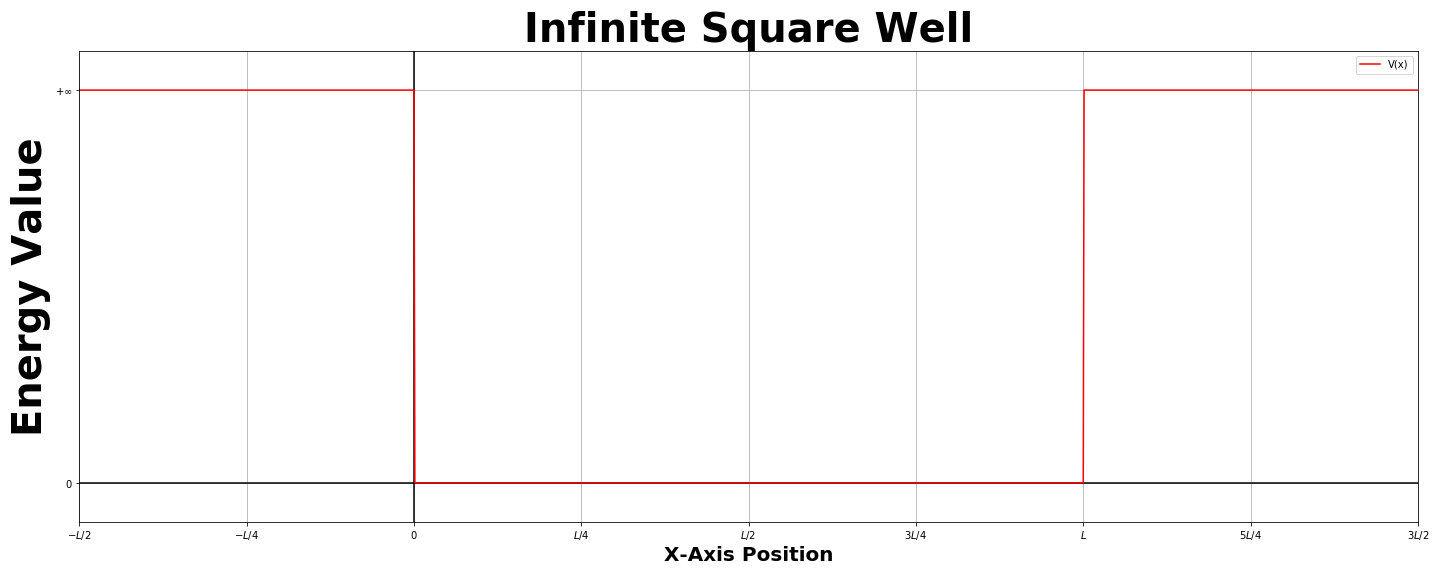
\includegraphics[scale=0.3]{ISW}
\end{center}
\paragraph*{}Right off of that bat, this allows for some great simplifications. First off, no matter what, Our particle cannot exist in the region $x < 0$ or $x > L$ because of the infinite amount of energy required to get there. Therefore, this quantum mechanical particle can \textit{only} exist in the region $0 \geq x \leq L$. With this, can can focus all of our attention to this region of space. All of the rules outline in the previous chapters still apply, but now we only have this small region of space to worry about.
\paragraph*{}So for the region between $x = 0$ and $x = L$, the TISE reads:
\begin{equation}
\label{ISW TISE}
-\frac{\hbar^2}{2m}\frac{d^2 \psi}{dx^2} = E\psi
\end{equation}
Notice how the $V(x)\psi(x)$ term from equation (\ref{1D TISE}) is gone because $V(x) = 0$ in these bounds. Now, we actually have much simpler equation to solve. We can use some algebraic manipulation to rearrange equation (\ref{ISW TISE}) into something very familiar from classical physics.
\begin{equation}
\label{HO ODE}
\frac{d^2 \psi}{dx^2} = -\frac{2mE}{\hbar^2}\psi
\end{equation}
\paragraph{}This is the standard ordinary differential equation for a mass-spring or any sort of harmonic oscillator -like system. This comes up all of the time in classical physics and is usually formed by equating Newton's second law, to Hooke's Law of ideal springs.  For simplicity's sake, lets make the assertion that a new constant can be created: $k = \frac{\sqrt{2mE}}{\hbar}$. (Note that is relies on the assumption that $E$ must be a positive value.) This changes the differential equation to:
\begin{equation}
\frac{d^2 \psi}{dx^2} = -k^2\psi
\end{equation}
Which has the solution:
\begin{equation}
\psi(x) = \alpha e^{+ikx} + \beta e^{-ikx}
\end{equation}
Which thanks to \textit{Euler's Identity}, can be rewritten as:
\begin{equation}
\psi(x) = a \sin(kx) + b \cos(kx)
\end{equation}
\paragraph*{}Here, $a$ and $b$ are constants chose based on initial condition or boundary conditions. From chapter 1, we learned that the wave function, 
$\psi(x)$ must be continuous over all space, and must be continuously differentiable over all of space. Since the potential function itself is not continuous differentiable (i.e. is peicewise defined), we can break this second rule. Regardless, since $\psi(x<0) = 0 $, and $\psi(x > L) = 0$, we can impose the boundary conditions on our system such that $\psi(x=0) = 0$ and $\psi(x=L) = 0$.
\paragraph*{}Applying these boundary conditions:
\begin{equation}
\psi(0) = a \sin(0) + b \cos(0) 
\text{\hspace*{8mm} and \hspace*{8mm}}
\psi(L) = a \sin(kL) + b \\cos(kL)
\end{equation}
Because of the nature of the sine and cosine functions, the only way for these equations to hold true is one of two ways. If $a = b = 0$, the whole wave function becomes $\psi(x) = 0$ which is a valid solution to the PDE, but not normalizeable, thus conflicts with one of our rules. Hence, the other option, just $b = 0$ is the valid conclusion. The resulting wave function for the infinite square well of width $L$ is:
\begin{equation}
\psi(x) = a \sin(kx) = a \sin\big(\frac{\sqrt{2mE}}{\hbar}x\big)
\end{equation}
\begin{flushright}
Where $kx$ must be an integer multiple of $\pi$: $kx = \pm \pi , \pm 2\pi , \pm 3\pm , ... , \pm n\pi , ...$
\end{flushright}
\paragraph*{}Because of the rotational symmetry of sine, ($-\sin(\theta) = +\sin(\theta)$), the negative integers become redundant, and since the function must fit "neatly" into a region $L$, the distinct solutions to the problem become:
\begin{equation}
\label{ISW spatial solution}
\psi_n(x) = A\sin \Big( \frac{n\pi}{L}x \Big)
\end{equation}
\paragraph*{}These $n$ functions are the \textit{energy eigenstates} to this problem and can be notated with kets: $\psi_n(x) = \ket{\psi_n}$. Just as presribebed by the equivalent eigenvalue problem, each eigenstate is appropriately orthonormal to the other eigenstates. 

% ================================

\section{The Finite Square Well}

% ================================

\section{Multiple Square Wells}


% ================================

\section{The Harmonic Oscillator}


% ================================

\section{The Free Particle}


% ================================

\section{The Delta Function}


% ================================


% ================================================================
% ================================================================

\chapter{The Rules of the Game}

% ================================================================

% ================================================================

% ================================================================

% ================================================================

% ================================================================
% ================================================================

\chapter{Mathematical Index}

% ================================================================
% ================================================================

\end{document}